\documentclass{beamer}
\usepackage[utf8]{inputenc}
\usepackage[T1]{fontenc}
\usepackage{ragged2e}
\justifying

\newcommand{\logoWidth}{1 cm}
\newcommand{\spaceh}{0,5 cm}


 \title{Automatic exploit generation}
\author[shortname]{
Maxime Bélair  \inst{1} \and
Manh-Dung Nguyen  \inst{2} \and
Emilien Fournier \inst{3}\and
 Tristan Benoit \inst{4}\and
Gabriel Sauger \inst{5}\\
\vspace{0.3cm}
\textbf{Subject by}: \large Jules Villard - 

\includegraphics[width = 1cm]{Figures/Logos/FacebookLogo.png}
}

\institute{
\inst{1}%
Orange Labs / IMT atlantique - \tiny maxime.belair@imt-atlantique.fr
\and
\inst{2}%
CEA LIST \& Université Grenoble Alpes - \tiny manh-dung.nguyen@cea.fr
\and
\inst{3}%
ENSTA Bretagne / Lab-STICC - \tiny emilien.fournier@ensta-bretagne.org
\and
\inst{4}%
LORIA - \tiny tristan.benoit@loria.fr
\and
\inst{5}%
LORIA - \tiny gabriel.sauger@loria.fr
}
\date{}

\titlegraphic{ \vspace{-1cm}


\includegraphics[width = \logoWidth]{Figures/Logos/MaxLogo1.png}

\includegraphics[width = 0.5cm]{Figures/Logos/MaxLogo2.png}
\hspace{\spaceh}

\includegraphics[width = 0.75cm]{Figures/Logos/MDLogo1.png}

\includegraphics[width = \logoWidth]{Figures/Logos/MDLogo2.png}
\hspace{\spaceh}

\includegraphics[width = 2.5cm]{Figures/Logos/EmilienLogo1.png}
\hspace{0.5cm}

\includegraphics[width = 2CM]{Figures/Logos/GabrielLogo1.png}
\hspace{\spaceh}
}


\usetheme{Antibes}


\setbeamertemplate{footline}[frame number]


\begin{document}

\begin{frame}
\titlepage
\end{frame}


\section{Problem overview}

\begin{frame}
\centering
\LARGE
Problem Overview
\end{frame}

\subsection{Context}

\begin{frame}{Context}

\begin{itemize}
\item Bugs in devices
\item Are they weaknesses ?
\end{itemize}

\begin{figure}

\includegraphics[width = 2cm]{Figures/HeartbleedLogo.png}
\end{figure}

\begin{block}{Formal challenge}
Can we automatically turn static analysis reports into executable confirming the vulnerability of a program ?
\end{block}


\end{frame}

\subsection*{Section example}
\begin{frame}{Section example}
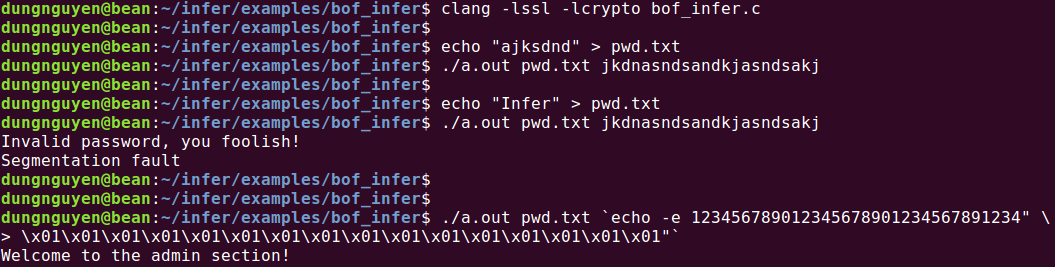
\includegraphics[width=12cm]{Figures/main.c/mainTest.png}
\end{frame}

\subsection{Infer tool}

\begin{frame}{Infer tool}

\begin{figure}
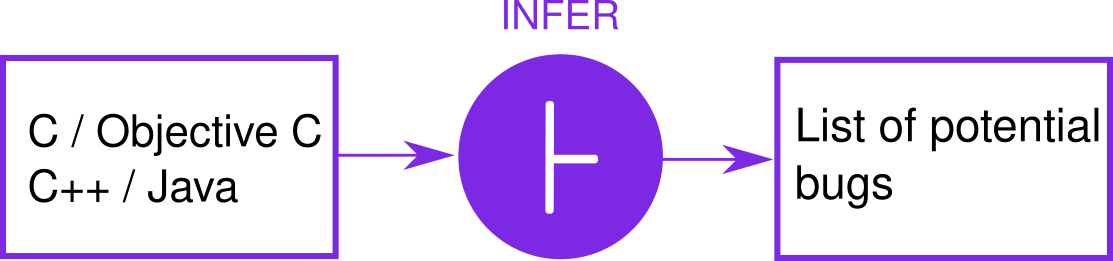
\includegraphics[width=10cm]{Figures/InferDrawing.png}
\end{figure}

\end{frame}

\begin{frame}

\begin{figure}

\includegraphics[width = 1.8cm]{Figures/InferLogo.png}

\end{figure}

\vspace{1cm}

\begin{itemize}
\item Static analysis tool from Facebook
\item \textbf{Capture} phase, then \textbf{Analysis} phase
\end{itemize}

\end{frame}

\begin{frame}{Infer tool example}

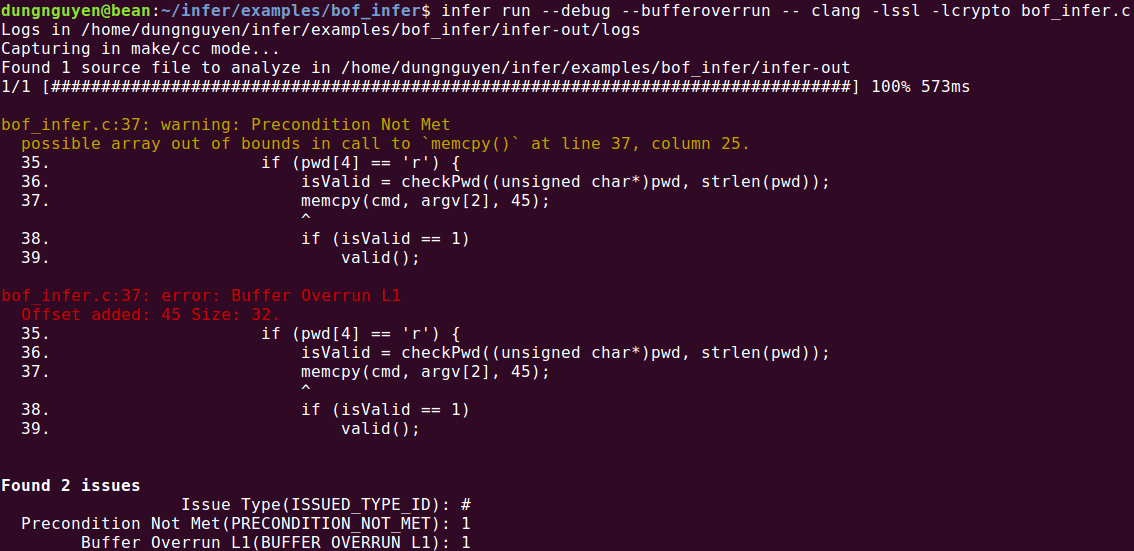
\includegraphics[width=12cm]{Figures/main.c/inferRunOnMain.png}
\end{frame}

\subsection{Practical approach}



\begin{frame}{Practical approach}

\includegraphics<1>[scale=0.3]{Figures/Workflow/1.png}
\includegraphics<2>[scale=0.3]{Figures/Workflow/2.png}
\includegraphics<3>[scale=0.3]{Figures/Workflow/3.png}
\includegraphics<4>[scale=0.3]{Figures/Workflow/4.png}

\end{frame}


\begin{frame}{Practical approach}

\begin{block}{Practical challenge}
Given the Infer information about bugs of a program A, create a program B that crashes A
\end{block}

\end{frame}

\begin{frame}{Table of content}
\tableofcontents
\end{frame}

\section{Proposed approaches}

\begin{frame}
\centering

P\LARGE roposed approaches
\end{frame}

\begin{frame}{Approaches overview}

\end{frame}

\subsection{Model checking}

\begin{frame}{Model checking }

    \begin{columns}
        \begin{column}{5cm}
 
            \begin{block}{ Overview }
                \begin{itemize}
                    \item Intuitive 
                    \item Automated 
                    \item Provides counter-examples 
                    \item[$\times$] State-space explosion
                \end{itemize}
            \end{block}
        
            \begin{block}{}
                \begin{itemize}
                    \item Fixed-point algorithm 
                    \item Plenty of algorithmic variations
                \end{itemize}
            \end{block}

        \end{column}
            
        \begin{column}{5cm}
            % \begin{block}{Overview}
                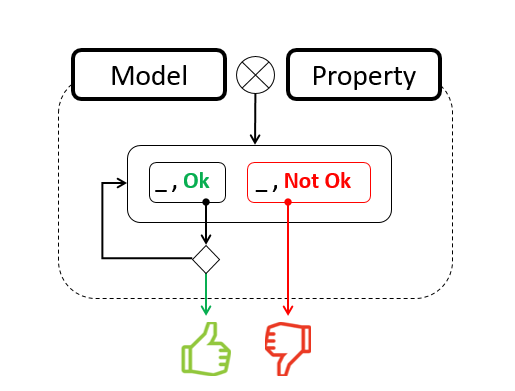
\includegraphics[width=\textwidth]{Figures/Model-checking.png}
            % \end{block}
        \end{column}
    \end{columns}
\end{frame}


\begin{frame}
    \frametitle{Application : How ? }

    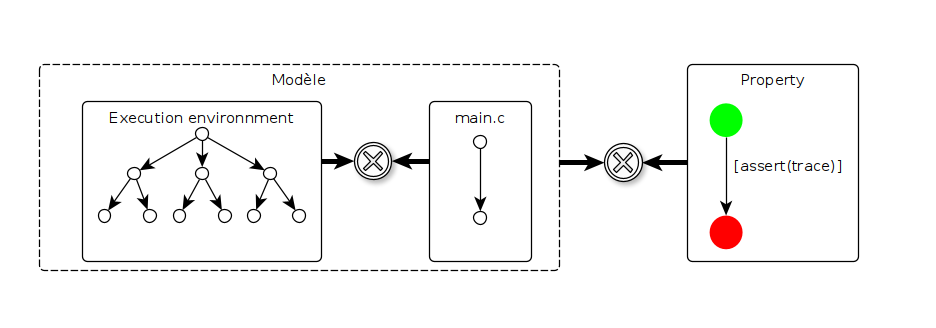
\includegraphics[width=\textwidth]{Figures/slide_mc.png}

    \begin{block}<>{Results}<>
        \begin{itemize}
            \item Custom model-checker
            \item 16 reachability algorithms supported
        \end{itemize}
    \end{block}

\end{frame}




\subsection{SMT solvers}

\begin{frame}{SMT solvers}

Present logic solvers

\end{frame}

\begin{frame}{SMT Solvers}
Compiler / Interpreter information
\end{frame}

\begin{frame}{SMT Solver}

\includegraphics<1>[width=9cm]{Figures/SMTsolver/1.png}
\includegraphics<2>[width=9cm]{Figures/SMTsolver/2.png}
\includegraphics<3>[width=9cm]{Figures/SMTsolver/3.png}
\includegraphics<4>[width=9cm]{Figures/SMTsolver/4.png}
\includegraphics<5>[width=9cm]{Figures/SMTsolver/5.png}
\includegraphics<6>[width=9cm]{Figures/SMTsolver/6.png}
\includegraphics<7>[width=9cm]{Figures/SMTsolver/7.png}

\end{frame}

\begin{frame}{SMT results}
Present the results we have and on which program. The performance review is NOT done here, but in Part 3/Result Comparison
\end{frame}

\subsection{Fuzzing technique}

\begin{frame}{Fuzzing technique}

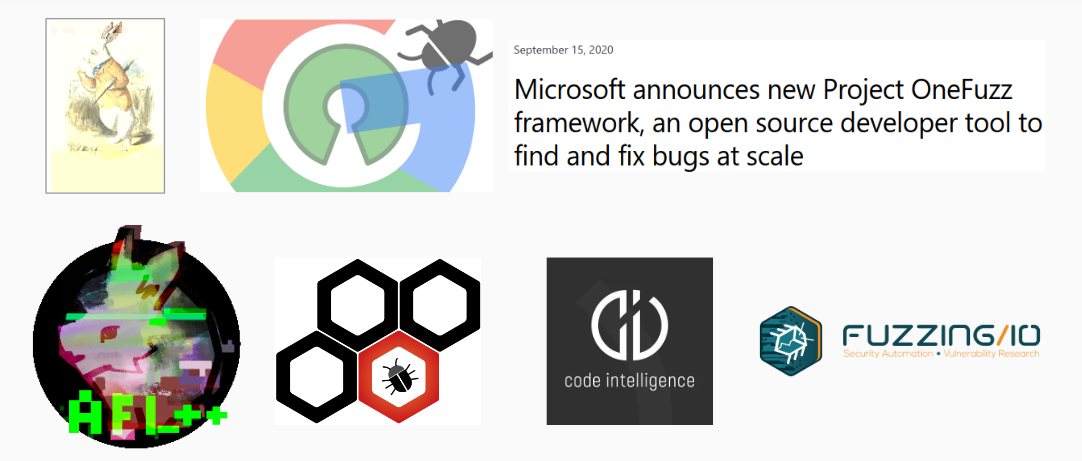
\includegraphics[width=11.5cm]{Figures/Fuzzing/graph1.png}

\end{frame}

\begin{frame}{Coverage-guided Greybox fuzzing}
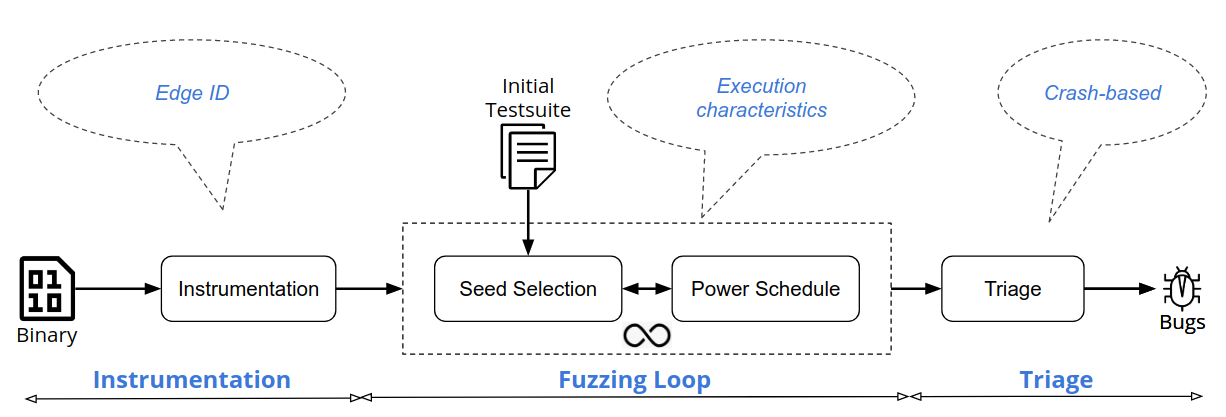
\includegraphics[width=11.5cm]{Figures/Fuzzing/graph2.png}
\end{frame}

\begin{frame}{Coverage-guided Greybox fuzzing}
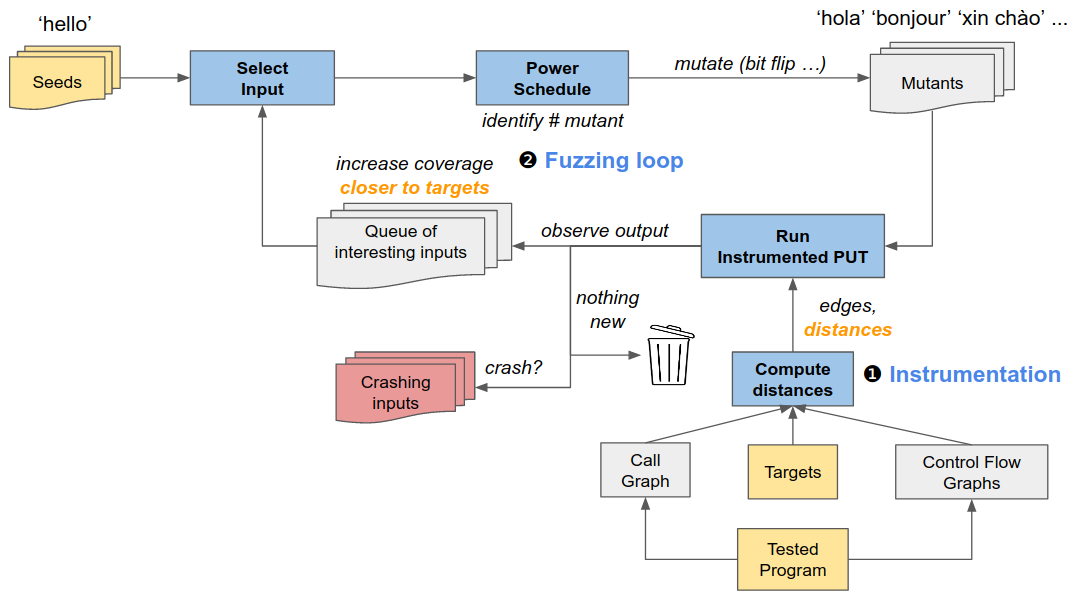
\includegraphics[width=11.5cm]{Figures/Fuzzing/graph3.png}
\end{frame}

\begin{frame}{Motivations}
Explain intuiton for our problem
\end{frame}

\begin{frame}{Fuzzing technique}

\includegraphics<1>[scale=0.3]{Figures/Fuzzing/1.png}
\includegraphics<2>[scale=0.3]{Figures/Fuzzing/2.png}
\includegraphics<3>[scale=0.3]{Figures/Fuzzing/3.png}
\includegraphics<4>[scale=0.3]{Figures/Fuzzing/4.png}
\includegraphics<5>[scale=0.3]{Figures/Fuzzing/5.png}

\end{frame}


\section{Conclusions and perspectives}

\begin{frame}
\centering
\LARGE Conclusions and perspectives
\end{frame}

\subsection{Results comparison}

\begin{frame}{Results comparison}

\textit{Show a table approaches / program comparing results (yes/no, running time, implementation complexity, computational complexity } \\

\end{frame}

\subsection{Future Work}
\begin{frame}{Future work}

Put eeeeeverything we think of. Ex:

\begin{itemize}
\item Create a fully automatic process
\item \textbf{SMT approach}: Manage fonctions calls in main.c 
\end{itemize}

\end{frame}

\begin{frame}{Future Work}
\textit{Add a graph of automatic exploits using expert models}
\end{frame}

\begin{frame}{Thank you Questions ?}

See the title

\end{frame}

\end{document}
